\section{Zadání}
(používejte: UTH0 = 0,4 V, KPn = 200 µA/V2, KPp = 50 µA/V2)

\begin{enumerate}
    \item Zlomte připravená multimodová vlákna
    \begin{enumerate}
        \renewcommand{\labelenumi}{\alph{enumi})}
        \item s pomocí lámačky vláken s diamantovým kotoučem
        \item s pomocí lámačky vláken s diamantovým nožem
        \item pomocí safírové destičky.
    \end{enumerate}
    \item Nastudujte nejpoužívanější metody spojování vláken a zapojte vámi zlomené vlákno do optické trasy pomocí rozebíratelného spoje.    
\end{enumerate}


\newpage
\section{Lámání Vláken}
  Nejprve je nutné optické vlákno zbavit ochrany, jak sekundární tak primární.
  To bylo provedeno pomocí přiložených kleští a následně bylo očištěno izopropyl alkoholem.
  
  \begin{figure}[h!]
    \centering
    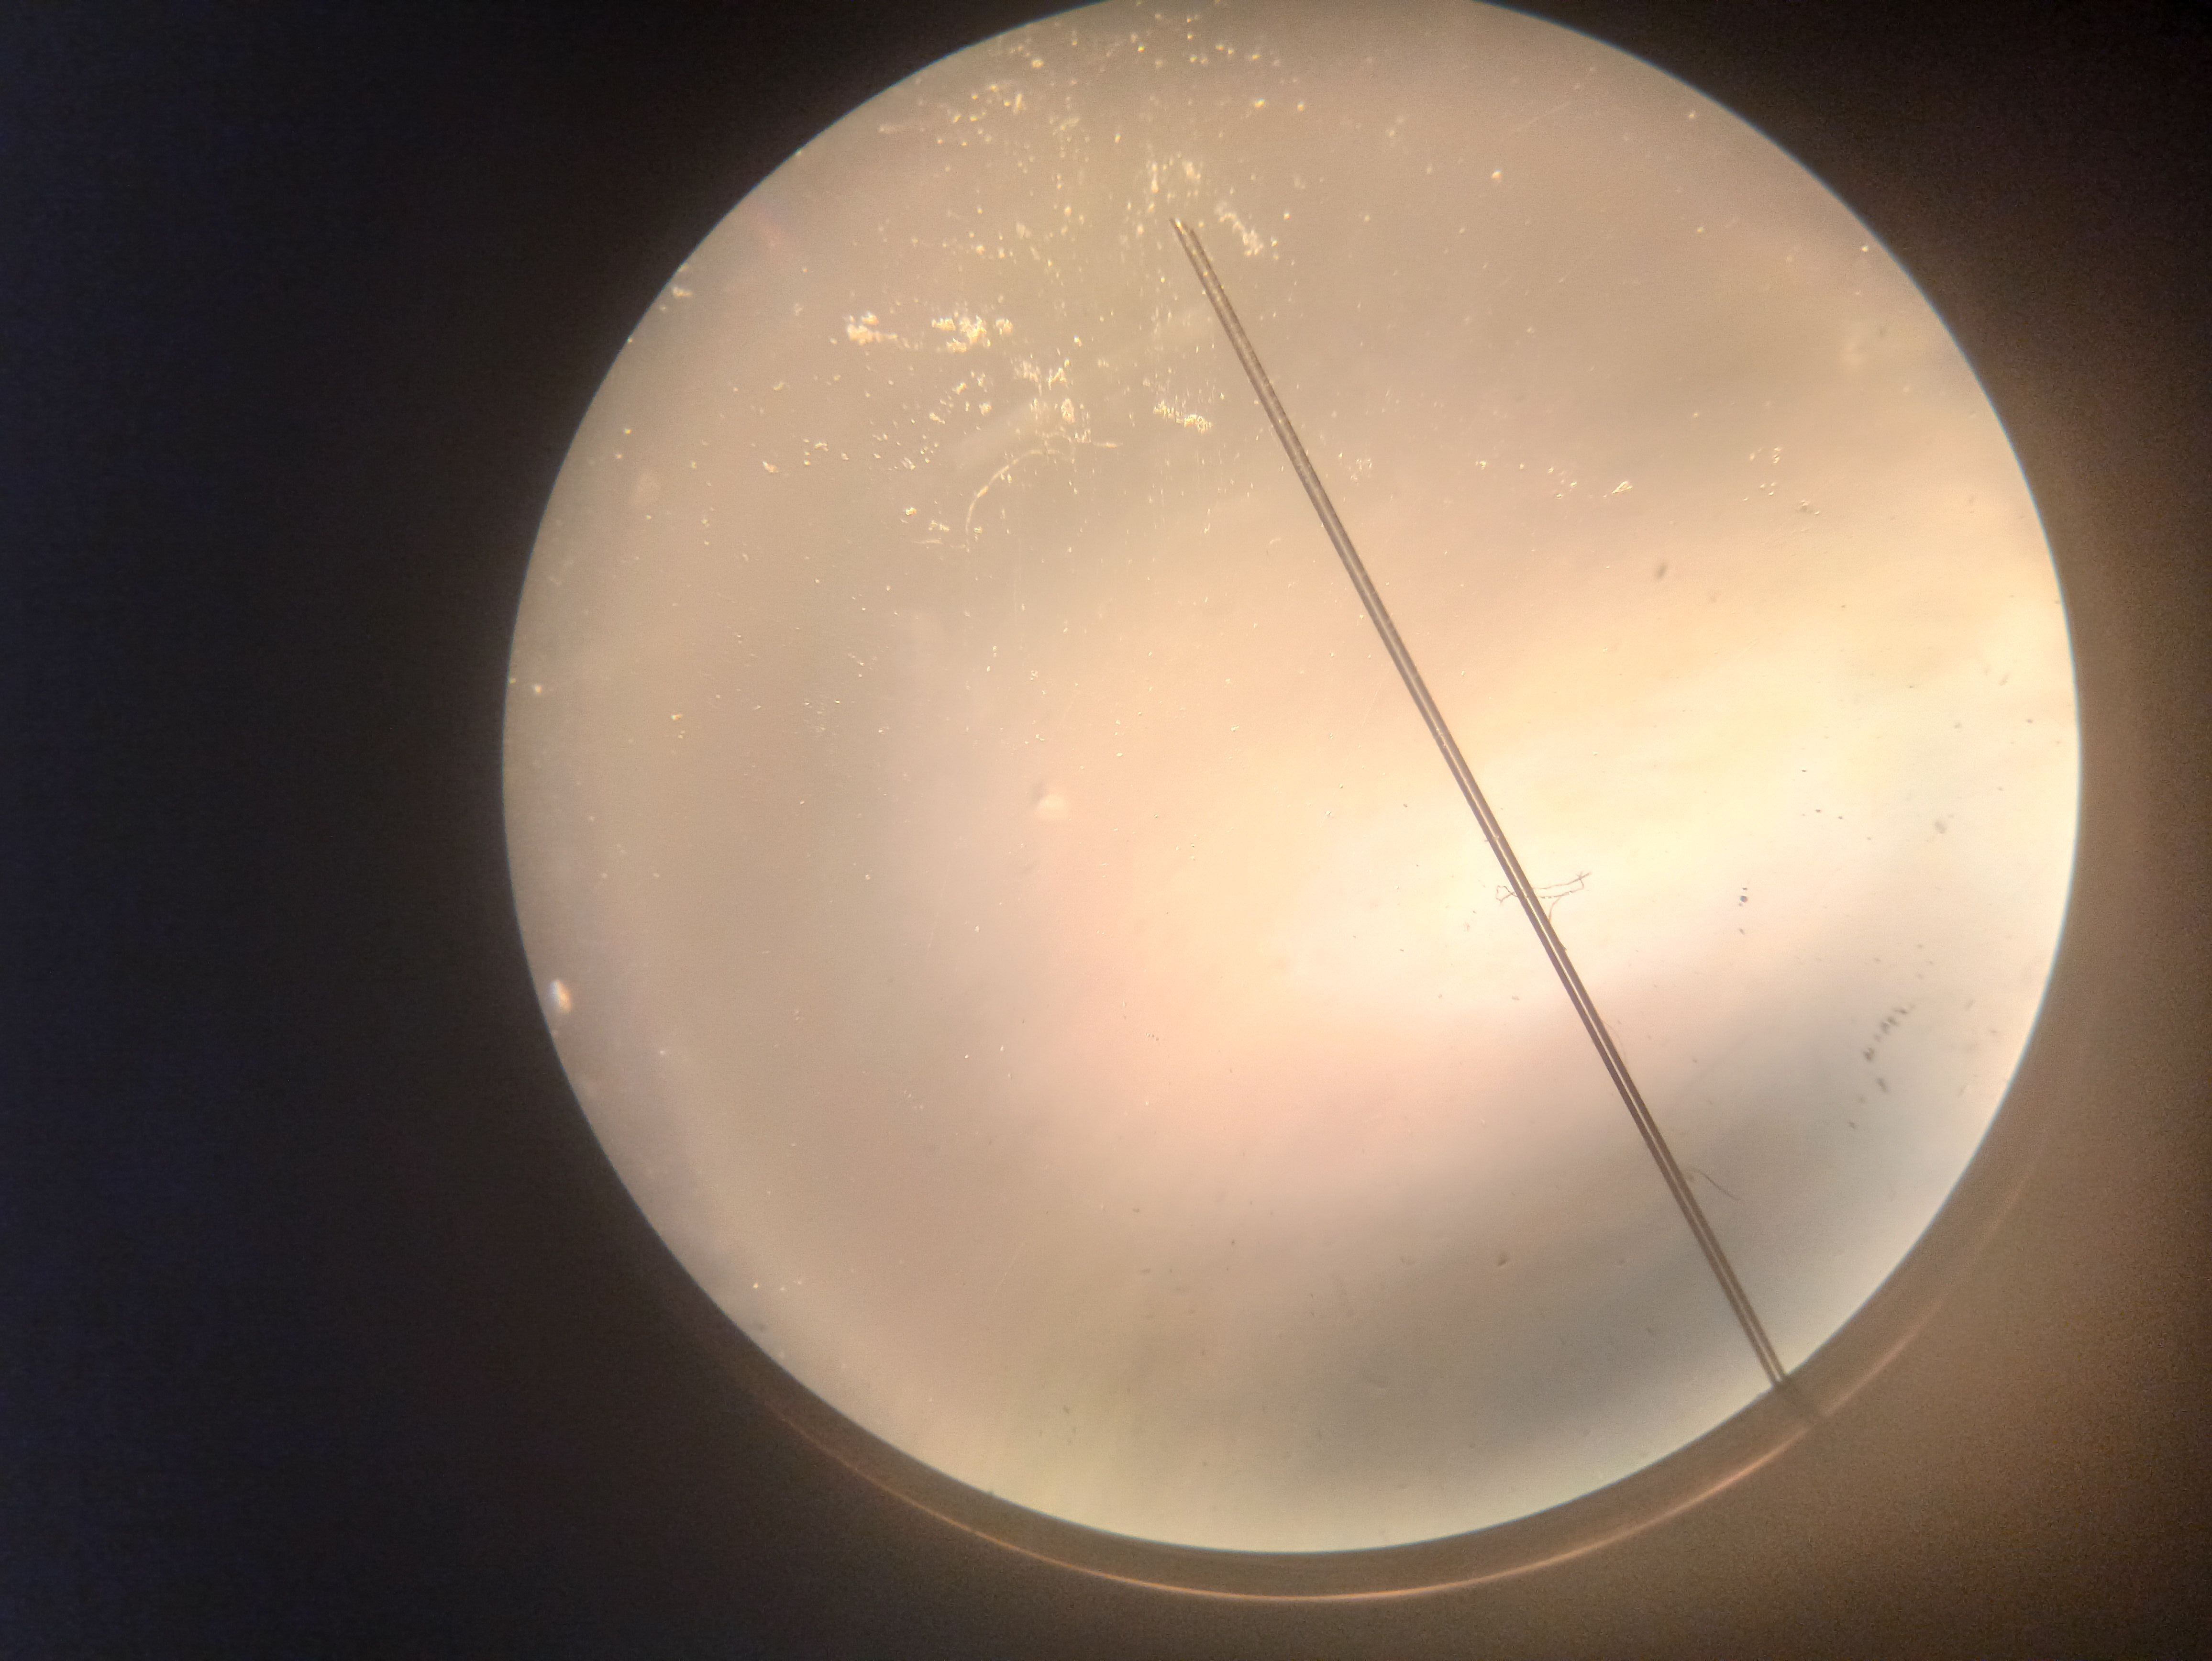
\includegraphics[width=0.6\textwidth]{text/img/odizolovano.jpg}
    \caption{\label{fig:odizolovano} Pohled mikroskopem na očištěné vlákno zbavené izolace}
  \end{figure}
  
  \subsection{Lámačka s diamantovým kotoučem}
    Vlákno zbavené ochrany bylo vloženo do lámačky a zlomeno.
    Následně bylo opět vloženo pod mikroskop, výsledek je viditelný na obrazcích \ref{fig:diamKot} a \ref{fig:diamKot_O}
    Jak je vidět, výsledný lom nedosahuje dostatečné kvality pro optický spoj, a ani po opakovaném pokusu se výsledek znatelně nezlepšil.  

    \begin{figure}[h!]
      \centering
      \includegraphics[width=0.6\textwidth]{text/img/diamantovyKotouc.jpg} 
      \caption{\label{fig:diamKot} Pohled mikroskopem na vlákno zlomené diamantovým kotoučem}
    \end{figure}

    \begin{figure}[h!]
      \centering
      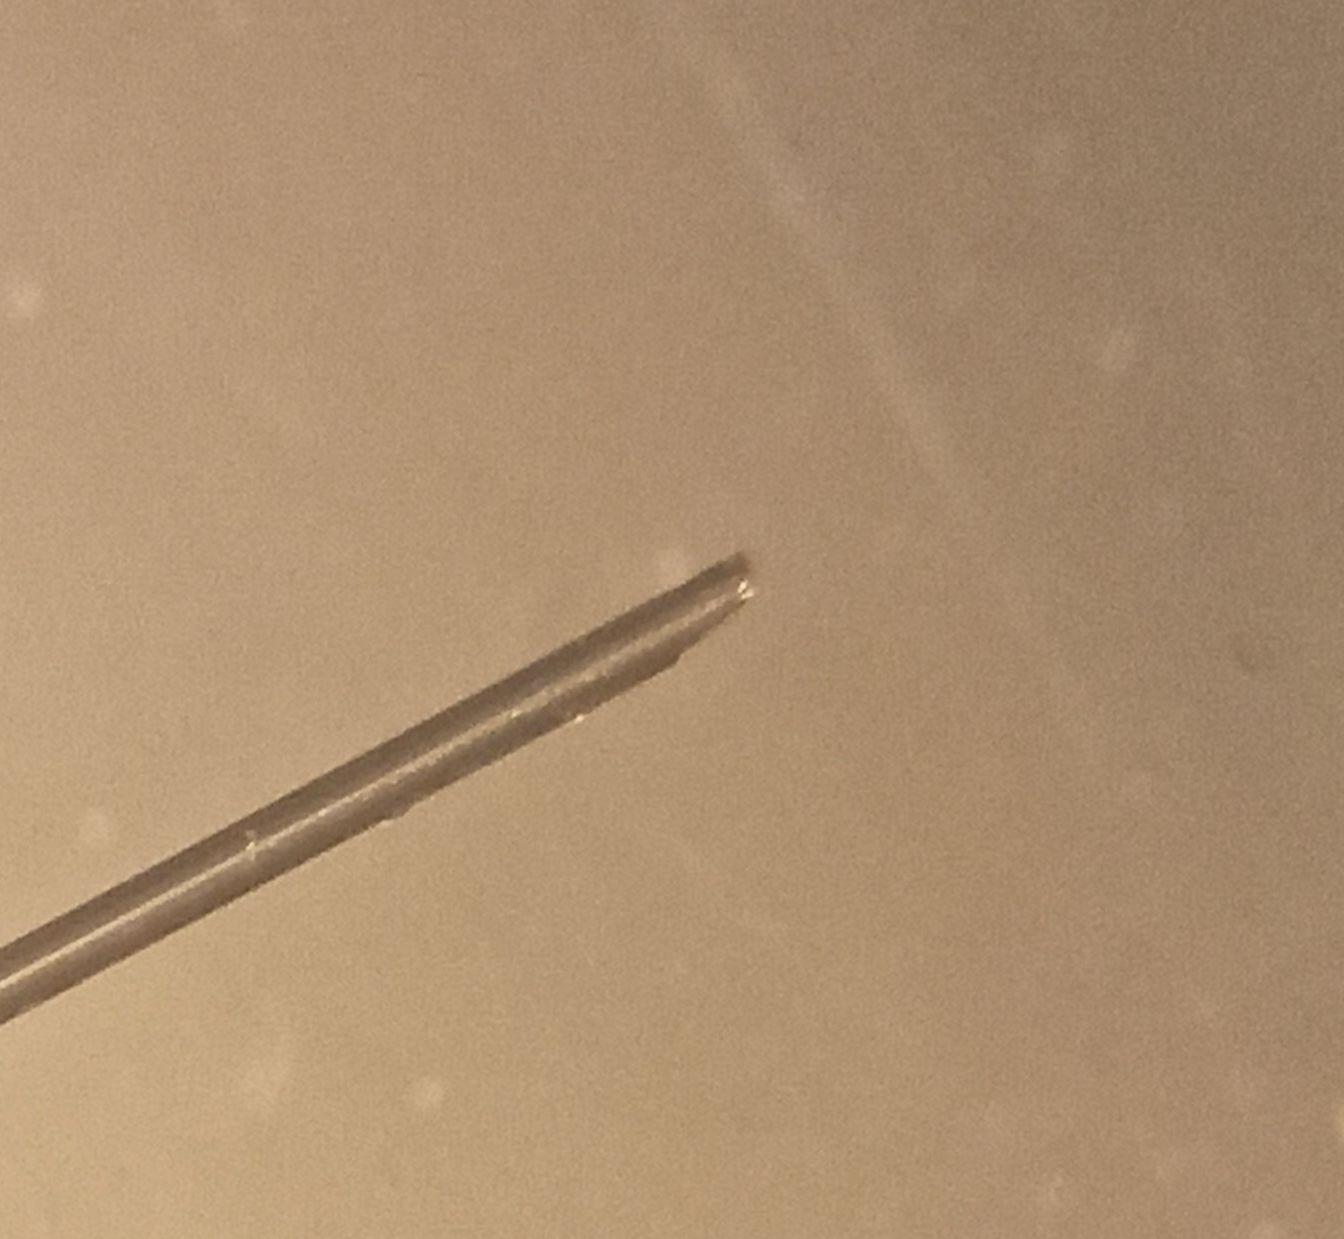
\includegraphics[width=0.6\textwidth]{text/img/diamantovyKotouc-O.jpg}
      \caption{\label{fig:diamKot_O} Oříznutý pohled na vlákno zlomené diamantovým kotoučem}
    \end{figure}

  \newpage
  \clearpage

  \subsection{Lámačka s diamantovým nožem}
    Obdobný postup byl aplikován u lámačky s diamantovým nožem.

    \begin{figure}[h!]
      \centering
      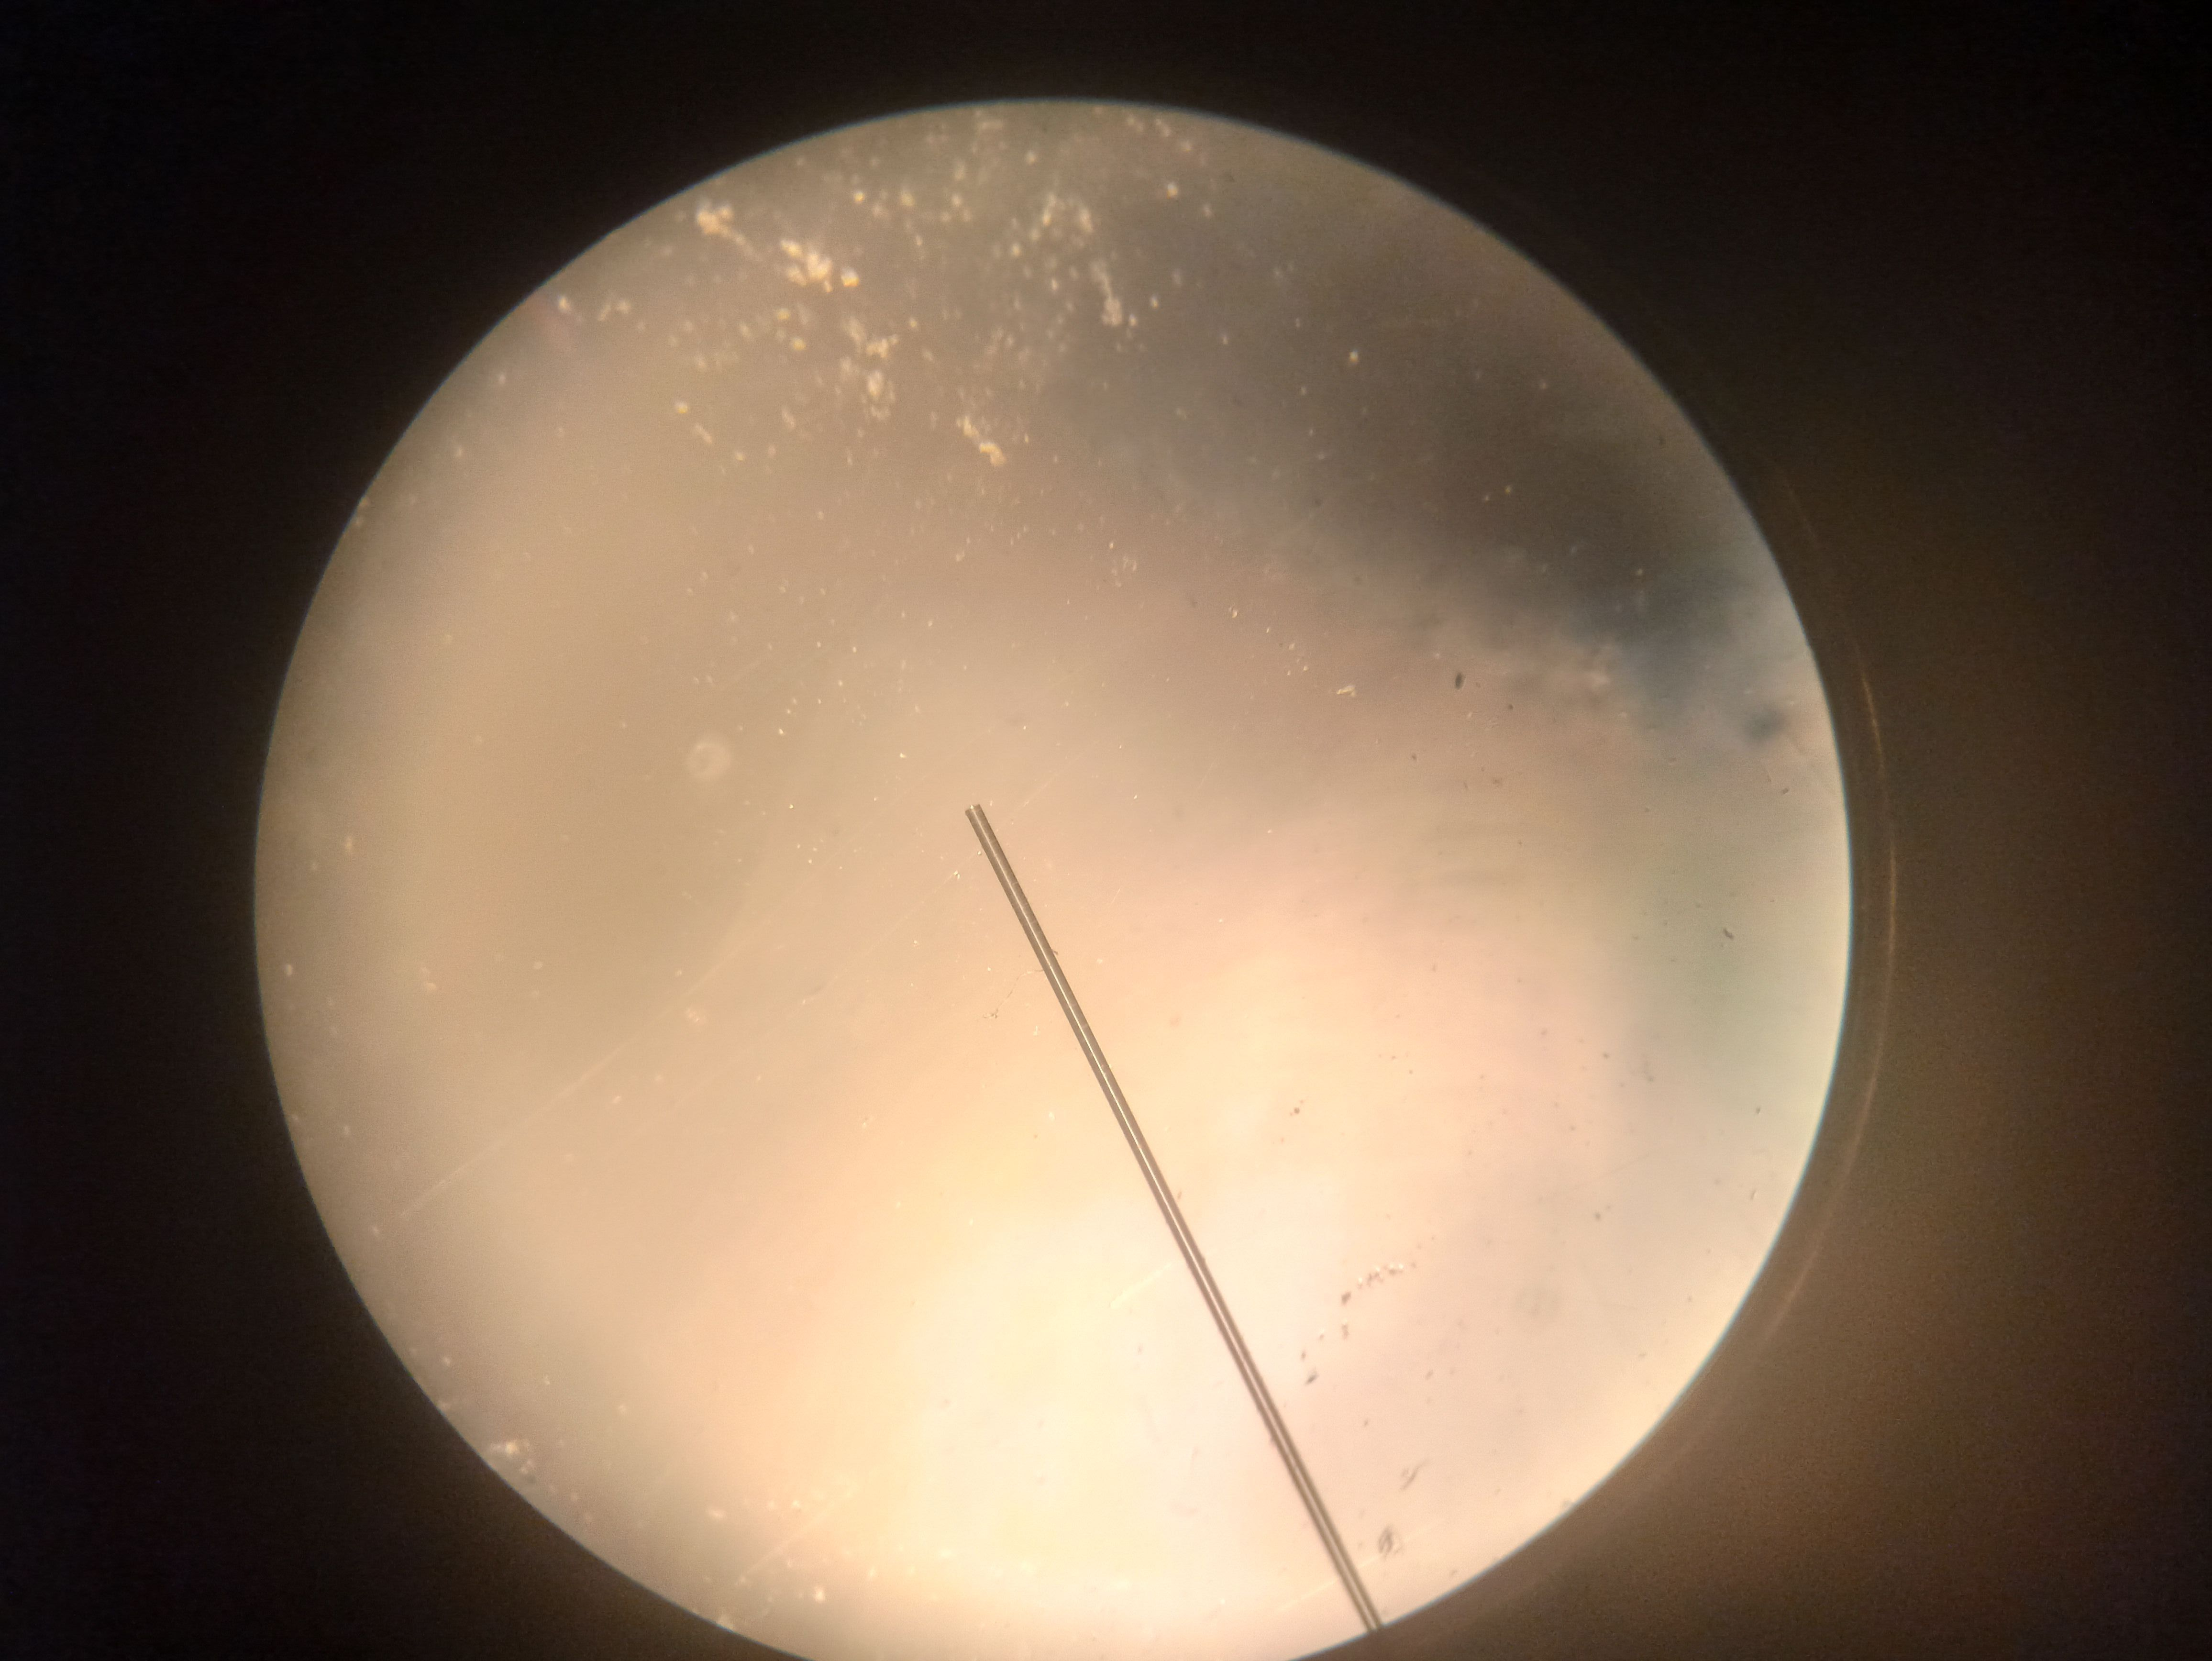
\includegraphics[width=0.6\textwidth]{text/img/diamantovyNuz.jpg} 
      \caption{\label{fig:diamNuz} Pohled mikroskopem na vlákno zlomené diamantovým nožem}
    \end{figure}

    \begin{figure}[h!]
      \centering
      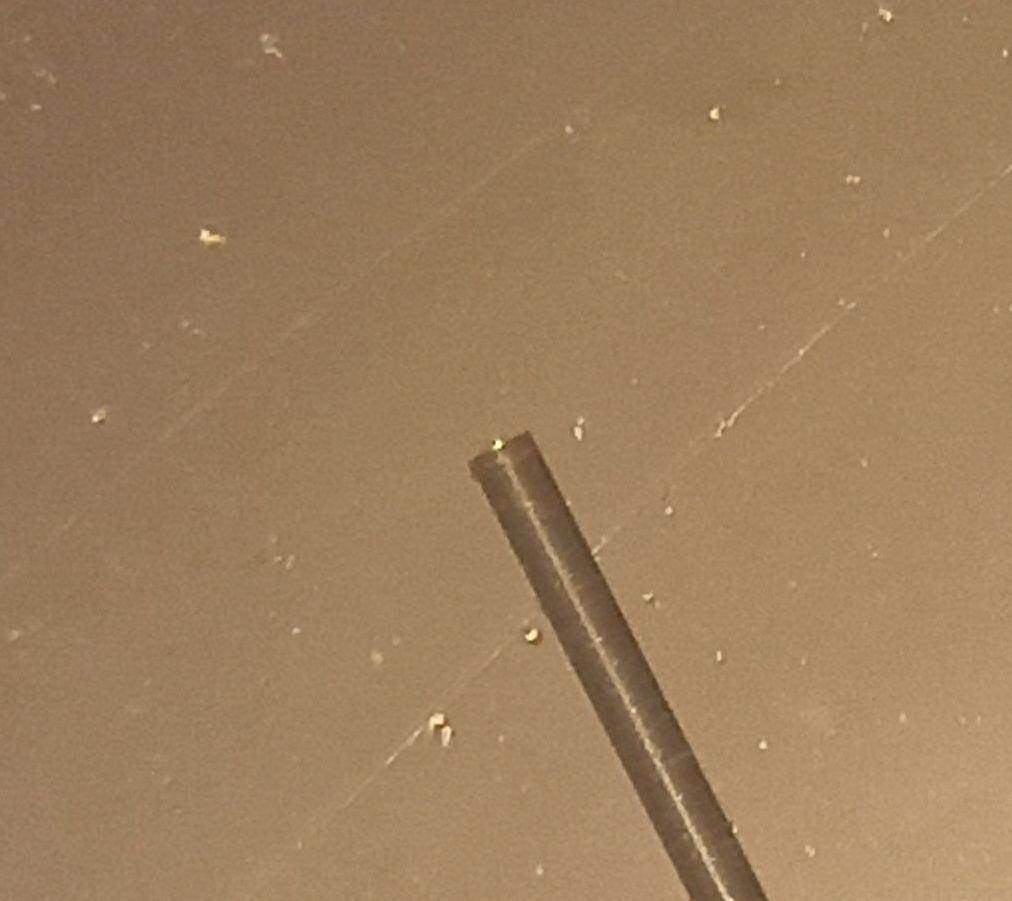
\includegraphics[width=0.6\textwidth]{text/img/diamantovyNuz-O.jpg}
      \caption{\label{fig:diamNuz-O} Oříznutý pohled na vlákno zlomené diamantovým nožem}
    \end{figure}

  \newpage
  \clearpage
  
  \vspace{-3mm}
  
  \subsection{Lom se safírovým nožem}
  
  \vspace{-3mm}

  \begin{figure}[h!]
    \centering
    \includegraphics[width=0.58\textwidth]{text/img/safirovyNuz.jpg} 
    \caption{\label{fig:safirNuz} Pohled mikroskopem na vlákno zlomené safírovým nožem}
  \end{figure}

  \vspace{-3mm}

  \subsection{Lom se safírovou destičkou}
    \vspace{-3mm}
    \begin{figure}[h!]
      \centering
      \includegraphics[width=0.58\textwidth]{text/img/safirovaDesticka2.jpg} 
      \caption{\label{fig:safirNuz} Pohled mikroskopem na vlákno zlomené safírovou destičkou}
    \end{figure}
  
  \vspace{-3mm}

  \section{Závěr}
  Jednotlivé metody lámání měly různé výsledky.
  Nejlépe se mi osvědčil diamantový nůž, který jako jediný vytvořil rovný kolmý řez.
  Nakontaktování se mi však nepodařilo vůbec. Signál procházející skrz spoj nebyl rozeznatelný od šumu, celý světelný výkon se tedy ztratil ve "spoji".